\chapter{Software Evolution in Real-world}
\label{chap:evolution}

The multi-version execution approach is based on two key assumptions.  First,
that new bugs are being introduced during the software evolution and
maintenance process even in well-tested code. Second, that during software
evolution, the externally observable behaviour of the applications remains
relatively stable, especially between minor revisions (\ie security and bug
fixes).  While there is a lot of first hand and anecdotal evidence in support
of these assumptions, despite the key role that software evolution plays in the
application life cycle, it is surprising how few empirical studies one can find
in the research literature regarding the evolution of the \emph{execution} of
real systems.

Software repositories provide rich information about the construction and
evolution of software systems. While static data extracted from software
repositories have been extensively studied, dynamic metrics concerning the
execution of the software have received much less attention, due to the
inherent difficulty of running and monitoring a large number of software
versions.

In this chapter, we present an empirical study concerning both static and
dynamic metrics which aims to answer some of the questions related to software
evolution. To perform this study, we have built a flexible infrastructure that
can be used to run each version of a system in isolation and collect static and
dynamic software metrics from the test suite execution. We consider the tests
to be an (imperfect) proxy for a real-world execution.

We have used this infrastructure to examine how code and tests co-evolve in
\numSystems popular open-source systems. We report the main characteristics of
software patches, and analyse the program evolution from both the source code
and the external behaviour perspective. We assess the impact of non-determinism
on the execution of test suites. We also analyse the code and patch coverage,
and investigate whether the coverage of code containing bugs and bug fixes is
lower or higher than average; the latter of the two would provide evidence that
even well tested code still has bugs, in support of our technique.

\begin{figure}[t!]
\centering
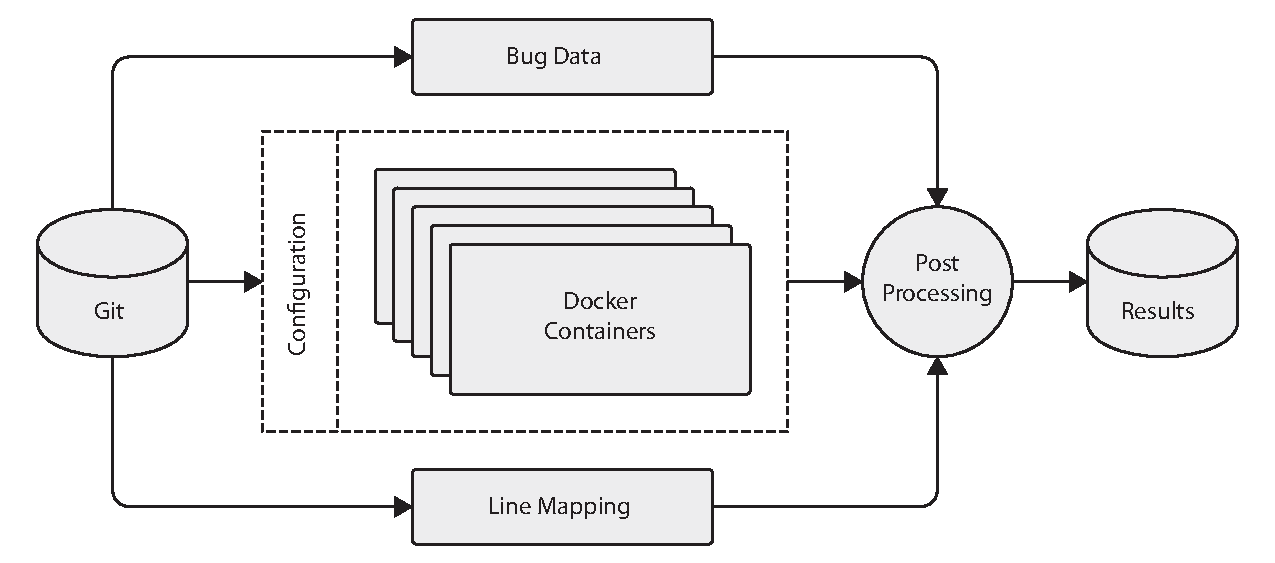
\includegraphics[width=\columnwidth]{evolution/figures/pipeline}
\caption{\covrig infrastructure.}
\label{fig:arch}
\end{figure}

The overall architecture of the \covrig infrastructure is depicted
in Figure~\ref{fig:arch}.  It contains a generic driver which
iterates through all the revisions in a given range and invokes
routines specific to each system to compile, run, and collect
statistics of interest.

%% To collect information about each program revision, such as whether it
%% successfully compiles, whether it passes the regression tests and with
%% what coverage, we built an infrastructure capable of automatically
%% retrieving and compiling each version of a target program, running
%% existing regression tests and collecting metrics of interest.

%The system is built on top of software containers~\cite{}, a
%lightweight virtualisation mechanism, which offers both isolation and
%reproducibility, by ensuring a consistent environment into which to
%run each software revision.  In this way, the execution of different
%revisions do not influence each other, \eg by inadvertently leaving
%behind lock files or not properly freeing up resources.

\paragraph{Lightweight software containers} \covrig employs software
containers~\cite{containers:eurosys07}, an operating system-level
virtualisation mechanism that provides the ability to run multiple
isolated virtual Linux systems (``containers'') inside a single host
OS.  When launched, \covrig starts by loading the selected range of
revisions from the project's \git repository, and for each revision
starts a new software container.  The use of containers offers
increased isolation and reproducibility guarantees by providing a
consistent environment in which to run each software revision and
ensuring that different revisions do not interfere with each other,
\eg by inadvertently leaving behind lock files or not properly freeing
up resources.

The choice of lightweight OS-level virtualisation rather than more
traditional virtual machines (\eg
\kvm\footnote{\url{http://www.linux-kvm.org/}} or
\xen\footnote{\url{http://www.xenproject.org/}}) reduces the
performance penalty associated with spawning and tearing down VMs,
operations performed for each revision analysed.  To get a sense of
this difference, we compared an
\lxc\footnote{\url{http://linuxcontainers.org/}} container, which
required under a second for these operations, with a \xen VM, which
needed over a minute.

In our implementation, we use
\docker\footnote{\url{https://www.docker.io/}} to create and manage
the lower-level \lxc containers, and
%Vagrant to
deploy them on multiple local or cloud machines.
Each container is used to configure, compile and test one
program revision, as well as collect the metrics of interest, such as
code size and coverage. The containers are remotely controlled through
SSH using the \fabric\footnote{\url{http://fabfile.org/}} framework.


\paragraph{Configuration file} \covrig has a modular architecture, which makes it
possible to analyse new systems with modest effort. A potential user
of our infrastructure only needs to provide a Python
configuration file describing the system.  A minimal file provides
the name of the system, its \git repository location, a method to
compile the system, \eg install dependencies and run the appropriate
\stt{make} command, and a method to run the regression tests, \eg run
the \stt{make test} command.
%
Finally, the configuration file can also specify an {\em end revision}
and a specific number of revisions to analyse.  
%% \covrig will use these parameters to determine the list of revisions to
%% analyse, independent of the target system's evolution.  
For accurate test suite size measurements, the files or folders which
make up the test suite can also be indicated.

For each revision, \covrig collects several static and dynamic metrics.  The
static metrics are obtained either directly from the version control
system (\eg the number of lines of test code) or after compiling each
revision (\eg the number of executable lines of code).  The dynamic
metrics require running the regression tests (\eg the overall line
coverage or the regression test success status).

Further information and graphs---including the ones presented in our
empirical study---are automatically derived in the post-processing
stage from these primary metrics using a set of scripts.

%% For example, we were able to verify that the {\em latent patch
%% coverage}, \ie the fraction of code which is executed only several
%% revisions after it is introduced is small, and practitioners can
%% safely ignore it most of the time when evaluating test suite
%% augmentation or coverage-improvement techniques.


%\subsection{Bug Data} \label{ssec:bugdesign}

\paragraph{Bug data} One possible application of \covrig is finding
useful data about software bugs and correlating them with the static
and dynamic metrics collected. For our study, we mined bug data from
both software repositories and, where available, bug tracking systems.
We automatically obtained a list of candidate bug-fixing revisions by
iterating through the list of commits and checking the commit message
for words such as {\em fix}, {\em bug} or {\em issue}, followed by a
number representing the bug identifier.  For example, a typical
\memcached bug fix commit message looks like {\em "Issue 224 - check
  retval of main event loop"}. The regular expression that we used to
identify these commits is similar to the ones used in prior
work~\cite{genealogies:issre13}:

\lstinline`(?:bug|issue|fix|resolve|close)\s*\#?\s?(\d+)`

Where possible, we confirmed that the bug identifier is valid by
querying the associated bug tracking system. We further manually
checked all reported revisions and confirmed that they included no
false positives.  While it is impossible to quantify the false
negative rate without a knowledgeable developer manually checking all
the revisions in a repository, we believe that the automatically
obtained bug fixes create a representative subset of the fixes in the
repository.

\paragraph{Line mapping} The ability to track how lines move and change
across revisions is the cornerstone of many high-level software
evolution analyses.  A line mapping algorithm improves over the
traditional \diff algorithm by tracking the movement of individual
lines rather than hunks.  Conceptually, line mapping is a function
which takes two revisions, \textit{r1} and \textit{r2}, and a program
location described by a pair \textit{(file name 1, line number 1)}
associated with \textit{r1}.  The output is a pair \textit{(file name
  2, line number 2)} identifying the corresponding location in
\textit{r2}.

Our implementation of the line mapping algorithm is similar to the
algorithms described in previous
work~\cite{szz:msr05,szz:ase06,change-source-code:msr07,szzrevisited:defects08}.
It makes use of the \emph{Levenshtein edit
  distance}~\cite{levenshtein1966binary} to track line edits, and
\emph{tf--idf}~\cite{tf-idf} and \emph{cosine
  similarity}~\cite{cosinesimilarity} to track line movements.  It
also uses the \emph{Hungarian algorithm}~\cite{hungarian} to find the
optimal matching of lines across versions.  Compared to previous work,
our implementation can also improve precision by using coverage information to filter
non-executable lines.

%% We used line mapping in two ways in our analysis: to determine whether
%% patches are tested within the next few revisions after they were
%% created (\S\ref{sec:lpcoverage}), and to estimate where bugs were
%% introduced (\S\ref{sec:bugs}).

In our study, we used line mapping to determine whether patches are
tested within the next few revisions after they were created
(\S\ref{sec:lpcoverage}).

\paragraph{Cloud deployment} To enable large-scale data collection and
processing, we deployed \covrig to our private cloud.  We have built our
system around a standard set of tools: Packer for building custom
Docker-enabled machine images, Vagrant for controlling and provisioning
the virtual machines based on these images, a Docker registry for
serving \covrig's Docker containers and a {\em fabfile} for
orchestrating the entire cluster. The same set of tools and scripts
can be used to deploy \covrig to different private or public clouds.

%% \subsection{High-Level Questions} \label{ssec:highlevel}

%% Coverage, bugs and line mapping data already provide useful insights into a
%% software project. For example, coverage and known bugs count can be used to
%% predict the residual bugs, i.e., the bugs still present in the software, using
%% a simple formula~\cite{coveragedefects98}

%% Using the bug data, we can quantify the number of patches which attempt to fix
%% a bug but either contain an incomplete fix or introduce new bugs. Such patches
%% are identified by looking for bug pairs, one being fixed and the other
%% introduced in the same patch. A high number of buggy fixes points to
%% deficiencies in the software development process.

%% \todo{More interesting things that we can do directly with coverage, bugs and
%% line mapping data}

%% However, further processing of this data allows us to answer more questions.
%% Combining  bug data and coverage data allows us to determine how many bugs are
%% in code which was already tested, i.e. executed without triggering the bug.
%% This may happen because the bug is only activated in corner-case scenarios.
%% Systems with a high number of bugs present in tested code may benefit from
%% symbolic execution-based testing tools such as ZESTI~\cite{zesti}, which
%% transparently instrument the existing tests to check for corner-case scenarios.
%% On the other hand, systems where the bugs are present in untested code can
%% benefit from test generation tools such as KATCH~\cite{katch}.

%% Correlations between bug data and software metrics can be used to build a bug
%% predictors based on project history and current patch coverage. Integrated in a
%% development environment or continuous integration system, such predictors can
%% warn developers when making high-risk changes. An intuitive predictor is based
%% on patch coverage: a tested patch is less likely to be buggy, compared to an
%% untested patch and the correlation can be mined from the project history. Code
%% churn can also be used as a predictor~\cite{churn-bugs:issre96, churndefects05}
%% and can be further refined to by eliminating non-executable changes or using
%% fine-grained souce code change extraction techniques~\cite{fluri:scc}
%% and its relationship with bugs can be mined using the line mapping data at the
%% line/function/file level.
%% % But we really don't want to go too much into statistics

%% Another question is whether old regression tests are still adequate for the
%% latest program version. We can quantify test adequacy by the fraction of the
%% code originally executed by the test that is still executed in the current
%% version. For an accurate computation we need to map the lines originally
%% executed to their counterparts in the current version.

\section{Overview}
\label{evolution:overview}

We used the our infrastructure to understand the evolution of \numSystems
popular open-source applications written in C/C++, over a combined period of
\numYears years. The \numSystems evaluated applications are:

\begin{enumerate}

\item[\gnu~\binutils\footnote{\url{http://www.gnu.org/software/binutils/}}]
is a set of utilities for inspecting and modifying object files,
libraries and binary programs.  We selected for analysis the twelve
utilities from the \stt{binutils} folder (\stt{addr2line}, \stt{ar},
\stt{cxxfilt}, \stt{elfedit}, \stt{nm}, \stt{objcopy}, \stt{objdump},
\stt{ranlib}, \stt{readelf}, \stt{size}, \stt{strings} and \stt{strip}),
which are standard user-level programs under many UNIX distributions.

\item[\beanstalkd\footnote{\url{http://kr.github.io/beanstalkd/}}]
is a simple and fast work queue originally designed for reducing the latency of
page views in high-volume web applications.

\item[\git\footnote{\url{http://git-scm.com/}}]
is one the most popular distributed version control systems used by the
open-source developer community.

\item[\lighttpd\footnote{\url{http://www.lighttpd.net/}}]
is a lightweight web server optimized for high performance environments.

\item[\lighttpdtwo\footnote{\url{http://redmine.lighttpdtwo.net/projects/lighttpdtwo2/}}]
is the new major version of the \lighttpd web server developed entirely from
scratch by the same team of developers.

\item[\memcached\footnote{\url{http://memcached.org/}}]
is a general-purpose distributed memory caching system used by several popular
sites such as Craigslist, Digg and Twitter.

\item[\redis\footnote{\url{http://redis.io/}}]
is a popular key-value data store used by many well-known services such as
Twitter, GitHub and StackOverflow.

\item[\vim\footnote{\url{http://www.vim.org/}}] is arguably one of the most
popular text editors.

\item[\zeromq\footnote{\url{http://zeromq.org/}}]
is a high-performance asynchronous messaging middleware library used by a
number of organisations such as Los Alamos Labs, NASA and CERN.

%\item {\bf GNU diffutils} is a collection of four widely-used
%programs: \stt{diff}, \stt{sdiff}, \stt{diff3} and \stt{cmp}, part of
%many popular UNIX distributions.

\end{enumerate}

The \numSystems applications are representative for C/C++ open-source code: GNU
\binutils are user-level utilities, \git is a version control system,
\beanstalkd, \lighttpdtwo, \memcached and \redis are server applications, \vim
is a text editor while \zeromq is a library.  All applications include a
regression test suite.

\begin{table}[t]
\caption{Summary of applications used in our study.
\textit{ELOC} represents the number of executable lines of code and
\textit{TLOC} the number of lines in test files in the last revision
analysed.}
\begin{center}
\begin{tabular}{llrlr}
\toprule
\multicolumn{1}{c}{}     & \multicolumn{2}{c}{\sc Code}& \multicolumn{2}{c}{\sc Tests} \\
\cmidrule(r){2-3}\cmidrule(l){4-5}
\textsc{Application} & \textsc{Language} & \textsc{ELOC} & \textsc{Language} & \textsc{TLOC}          % & \bf Time         
\\ \midrule
\beanstalkd  & C         & \beanstalkdSize & C        & \beanstalkdTsize  % & \beanstalkdTestTime
\\
\binutils    & C         & \binutilsSize  & DejaGnu   & \binutilsTsize    % & \binutilsTestTime 
\\
\git         & C         & \gitSize       & C/shell   & \gitTsize         % & \gitTestTime 
\\
\lighttpd    & C         & \lighttpdSize  & Perl    & \lighttpdTsize    % & \lighttpdtwoTestTime 
\\
\lighttpdtwo    & C         & \lighttpdtwoSize  & Python    & \lighttpdtwoTsize    % & \lighttpdtwoTestTime 
\\
\memcached   & C         & \memcachedSize & C/Perl    & \memcachedTsize   % & \memcachedTestTime 
\\
\redis       & C         & \redisSize     & Tcl       & \redisTsize       % & \redisTestTime    
\\
\vim         & C         & \vimSize       & Vim script       & \vimTsize      % & \vimTestTime   
\\
\zeromq      & C++       & \zeromqSize    & C++       & \zeromqTsize      % & \zeromqTestTime   
\\ \bottomrule
\end{tabular}
\end{center}
\label{tbl:study-systems}
\end{table}

\subsection{Basic characteristics}

Table~\ref{tbl:study-systems} shows some basic characteristics of these
systems: the language in which the code and tests are written, the number of
executable lines of code (ELOC) and the number of lines of test code (TLOC) in
the last revision analysed. To accurately measure the number of ELOC, we
leveraged the information stored by the compiler in \texttt{gcov} graph files,
while to measure the number of TLOC we did a simple line count of the test
files (using \texttt{cloc}, or \texttt{wc~-l} when \texttt{cloc} cannot detect
the file types).

The code size for these applications varies from only \memcachedSize ELOC for
\memcached to \gitSize ELOC for \git.  The test code is written in a variety of
languages and ranges from \lighttpdtwoTsize lines of Python code for
\lighttpdtwo to \gitTsize lines of C and shell code for \git.  The test code is
36\% larger than the application code in the case of \git, approximately as
large as the application code for \memcached, around 40\% of the application
code for \redis and \zeromq, and only around 10\% and 19\% of the application
code for \lighttpdtwo, \vim and \binutils respectively.  Running the test suite
on the last version takes only a few seconds for \binutils, \lighttpdtwo, \vim
and \zeromq, \memcachedTestTime seconds for \memcached, \redisTestTime seconds
for \redis, and 30 minutes for \git, using a four-core Intel Xeon E3-1280
machine with 16 GB of RAM.

The version control system used by majority of these applications is \git.
Four of these projects---\git, \memcached, \redis, and \zeromq ---are hosted on
the \github\footnote{\url{https://github.com/}} online project site.  The other
two---\binutils and \lighttpdtwo---use their own \git hosting. \lighttpd uses
Subversion, but the project also provides a \git mirror on \github. \vim uses
Mercurial.

\subsection{Selection of revisions}

Our goal was to select a comparable number of revisions across applications.
The methodology was to start from the current version at the day of our
experiments, and select an equal number of previous revisions for all systems.
We only counted revisions which modify executable code, tests or both because
this is what our analyses look at. We decided to select 250 such revisions from
each system because some systems had non-trivial dependency issues further back
than this, which prevented us from properly compiling or running them.  We
still had to install the correct dependencies where appropriate, \eg downgrade
\stt{libev} for older versions of \lighttpdtwo and \stt{libevent} for
\memcached.

Note that not all revisions compile, either due to development errors
%(an example of this would be someone forgetting to add a file) 
or portability issues (\eg system header files differing across OS
distributions).
%% Note that we distinguish between this kind of permanent errors (which
%% disallow us to compile all versions earlier than some revision) and
%% more transient compilation errors that affect only some program
%% versions.  
Redis has the largest number of such transient compilation
errors---\redisTransientCompErrs.  The prevailing reasons are missing
\stt{\#include} directives, \eg \stt{unistd.h} for the \stt{sleep} function,
and compiler warnings subsequently treated as errors.  The missing
\stt{\#include} directives most likely slipped past the developers because on
some systems other \stt{libc} headers cause the missing headers to be
indirectly included. The compiler warnings were generated because newer
compiler versions, such as the one that we used, are more pedantic.  Other
reasons include forgotten files and even missing semicolons.

We decided to fix the errors which had likely not been seen at the time a
particular revision was created, for example by adding the compile flag
\stt{-Wno-error} in \binutils so that warnings do not terminate the build
process. In all situations when we could not compile a revision, we rolled over
the changes to the next revisions until we found one where compilation was
successful.  Revisions which do not successfully compile are not counted
towards the 250 limit.

Another important decision concerns the granularity of the revisions
being considered.  Modern decentralised software repositories based on
version control systems such as \git do not have a linear structure
and the development history is a directed acyclic graph rather than a
simple chain.  Different development styles generate different
development histories; for example, \git, \redis and \zeromq exhibit a
large amount of branching and merging while the other three systems
have a mostly linear history.  Our decision was to focus on the main branch,
and treat each merge into it as a single revision. In other words, we
considered each feature branch a single indivisible unit.  Our
motivation for this decision was twofold: first, development branches
are often spawned by individual developers in order to work on a
certain issue and are often ``private'' until they are merged into the
main branch.  As a result, sub-revisions in such branches are often
unusable or even non-compilable, reflecting work-in-progress.  Second,
the main branch is generally the one tracked by most users, therefore
analysing revisions at this level is a good match in terms of
understanding what problems are seen in the field.  This being said,
there are certainly development styles and research questions that would
require tracking additional branches; however, we believe that for our
benchmarks and research questions this level of granularity provides meaningful
answers.

% On a secondary note, we remark that an additional complication with
% this approach is that version control systems do not associate a
% branch name to each revision, so some detective work might be required
% to follow the main development branch.  However, since
% the projects exhibiting a branching structure are hosted on \github, an implicit central
% integrator exists (the project owner) and we considered their history
% to be the official one, essentially always following the first parent
% in a merge.

\begin{table}[t]
\centering
\caption{Revisions used in our study.
  {\em OK}:~code compiles and tests complete successfully,
  {\em TF}:~some tests fail,
  {\em TO}:~tests time out,
  {\em CF}:~compilation fails,
  {\em Time}:~the number of months analysed.}
\begin{tabular}{lrrrrr}
\toprule
\multicolumn{1}{c}{}          &       \multicolumn{3}{c}{\sc OK+TF+TO=250}                 &            \multicolumn{2}{c}{}                   \\
\cmidrule{2-4}
\textsc{Application} & \textsc{OK} & \textsc{TF} & \textsc{TO} & \textsc{CF} & \textsc{Time}           \\
\midrule
\beanstalkd  &  \beanstalkdOK & \beanstalkdTransientTestErrs & \beanstalkdTransientTestTimeouts & \beanstalkdTransientCompErrs  &  {\beanstalkdTimespan}mo \\
\binutils    &  \binutilsOK   & \binutilsTransientTestErrs  & \binutilsTransientTestTimeouts  & \binutilsTransientCompErrs  &  {\binutilsTimespan}mo \\
\git         &  \gitOK        & \gitTransientTestErrs       & \gitTransientTestTimeouts       & \gitTransientCompErrs       &  {\gitTimespan}mo  \\
\lighttpd    &  \lighttpdOK   & \lighttpdTransientTestErrs  & \lighttpdTransientTestTimeouts  & \lighttpdTransientCompErrs  &  {\lighttpdTimespan}mo  \\
\lighttpdtwo    &  \lighttpdtwoOK   & \lighttpdtwoTransientTestErrs  & \lighttpdtwoTransientTestTimeouts  & \lighttpdtwoTransientCompErrs  &  {\lighttpdtwoTimespan}mo  \\
\memcached   &  \memcachedOK  & \memcachedTransientTestErrs & \memcachedTransientTestTimeouts & \memcachedTransientCompErrs &  {\memcachedTimespan}mo \\
\redis       &  \redisOK      & \redisTransientTestErrs     & \redisTransientTestTimeouts     & \redisTransientCompErrs     &  {\redisTimespan}mo     \\
\vim         &  \vimOK        & \vimTransientTestErrs       & \vimTransientTestTimeouts       & \vimTransientCompErrs    &  {\vimTimespan}mo    \\
\zeromq      &  \zeromqOK     & \zeromqTransientTestErrs    & \zeromqTransientTestTimeouts    & \zeromqTransientCompErrs    &  {\zeromqTimespan}mo    \\
\bottomrule
\end{tabular}
\label{tbl:revisions}
\end{table}


Table~\ref{tbl:revisions} summarises the revisions that we selected:
they are grouped into those that compile and pass all the tests (\emph{OK}),
compile but fail some tests (\emph{TF}), compile but time out while running the
test suite (\emph{TO}), and fail to compile (\emph{CF}).  The time limit that
we enforced was empirically selected for each system such that it is large
enough to allow a correct revision to complete all tests. As shown in the
table, timeouts were a rare occurrence, with at most one occurrence per
application.

Table~\ref{tbl:revisions} also shows the development time span
considered, which ranges from only 5-6 months for \git and \redis,
which had a fast-paced development during this period, to almost 4
years for \memcached. The age of the projects at the first version
that we analysed ranges from a little over 2 years for \lighttpdtwo,
to 11 years for \binutils.
%6 years memcached, 4 years redis, 2yr 9mo zeromq, 8 years git

\subsection{Revision setup}

All the programs analysed were compiled to record coverage information. In
addition, we disabled compiler optimisations, which generally interact poorly
with coverage measurements. We used existing build targets and configuration
options if available, otherwise we configured the application with the flags
\lstinline`CFLAGS='-O0 -coverage'` and \lstinline`LDFLAGS=-coverage`. All code
from the system headers, \ie \stt{/usr/include/} was excluded from the results.

Each revision was run in a virtualised environment based on 64-bit version of
Ubuntu 12.10 (12.04.3 for \git) running inside an \lxc container.  To take
advantage of the inherent parallelism of this approach, the containers were
spawned in one of 28 long-running \xen VMs, each with a 4~Ghz CPU, 6~GB of RAM,
and 20~GB of storage, running a 64-bit version of Ubuntu 12.04.3.

% The following sections present the main findings of our analysis.  They first
% reiterate and then examine in detail our target research questions (RQs).

We used the \covrig infrastructure to understand the evolution of
\numSystems popular open-source applications written in C/C++, over a
combined period of \numYears years. The six evaluated applications are:

\begin{enumerate}

\item[\gnu~\binutils\footnote{\url{http://www.gnu.org/software/binutils/}}]
is a set of utilities for inspecting and modifying object files,
libraries and binary programs.  We selected for analysis the twelve
utilities from the \stt{binutils} folder (\stt{addr2line}, \stt{ar},
\stt{cxxfilt}, \stt{elfedit}, \stt{nm}, \stt{objcopy}, \stt{objdump},
\stt{ranlib}, \stt{readelf}, \stt{size}, \stt{strings} and \stt{strip}),
which are standard user-level programs under many UNIX distributions.

\item[\beanstalkd\footnote{\url{http://kr.github.io/beanstalkd/}}] is a
  simple and fast work queue originally designed for reducing the latency of
  page views in high-volume web applications.

\item[\git\footnote{\url{http://git-scm.com/}}] is one the
most popular distributed version control systems used by the open-source
developer community.

\item[\lighttpdtwo\footnote{\url{http://redmine.lighttpdtwo.net/projects/lighttpdtwo2/}}]
is a lightweight web server optimized for high performance environments.
We examined version 2, which is the latest development branch.

\item[\memcached\footnote{\url{http://memcached.org/}}]
is a general-purpose distributed memory caching system used by several
popular sites such as Craigslist, Digg and Twitter.

\item[\redis\footnote{\url{http://redis.io/}}]
is a popular key-value data store used by many well-known
services such as Twitter, GitHub and StackOverflow.

\item[\zeromq\footnote{\url{http://zeromq.org/}}]
is a high-performance asynchronous messaging middleware library used by
a number of organisations such as Los Alamos Labs, NASA and CERN.

%\item {\bf GNU diffutils} is a collection of four widely-used
%programs: \stt{diff}, \stt{sdiff}, \stt{diff3} and \stt{cmp}, part of
%many popular UNIX distributions.

\end{enumerate}

The \numSystems applications are representative for C/C++ open-source
code: GNU \binutils are user-level utilities, \git is a version
control system, \beanstalkd, \lighttpdtwo, \memcached and \redis are server
applications, while \zeromq is a library.  All applications include a
regression test suite.

\begin{table}[t]
\caption{Summary of applications used in our study.
\textit{ELOC} represents the number of executable lines of code and
\textit{TLOC} the number of lines in test files in the last revision
analysed.}
\begin{center}
\begin{tabular}{llrlr}
\toprule
\multicolumn{1}{c}{}     & \multicolumn{2}{c}{\sc Code}& \multicolumn{2}{c}{\sc Tests} \\
\cmidrule(r){2-3}\cmidrule(l){4-5}
\textsc{Application} & \textsc{Language} & \textsc{ELOC} & \textsc{Language} & \textsc{TLOC}          % & \bf Time         
\\ \midrule
\beanstalkd  & C         & \beanstalkdSize & C        & \beanstalkdTsize  % & \beanstalkdTestTime
\\
\binutils    & C         & \binutilsSize  & DejaGnu   & \binutilsTsize    % & \binutilsTestTime 
\\
\git         & C         & \gitSize       & C/shell   & \gitTsize         % & \gitTestTime 
\\
\lighttpdtwo    & C         & \lighttpdtwoSize  & Python    & \lighttpdtwoTsize    % & \lighttpdtwoTestTime 
\\
\memcached   & C         & \memcachedSize & C/Perl    & \memcachedTsize   % & \memcachedTestTime 
\\
\redis       & C         & \redisSize     & Tcl       & \redisTsize       % & \redisTestTime    
\\
\zeromq      & C++       & \zeromqSize    & C++       & \zeromqTsize      % & \zeromqTestTime   
\\ \bottomrule
\end{tabular}
\end{center}
\label{tbl:systems}
\end{table}

\paragraph{Basic characteristics} Table~\ref{tbl:systems} shows some basic
characteristics of these systems: the language in which the code and tests are
written, the number of executable lines of code (ELOC) and the number of lines
of test code (TLOC) in the last revision analysed. To accurately measure the
number of ELOC, we leveraged the information stored by the compiler in
\texttt{gcov} graph files, while to measure the number of TLOC we did a simple
line count of the test files (using \texttt{cloc}, or \texttt{wc~-l} when
\texttt{cloc} cannot detect the file types).

The code size for these applications varies from only \memcachedSize
ELOC for \memcached to \gitSize ELOC for \git.  The test code is written in
a variety of languages and ranges from \lighttpdtwoTsize lines of Python
code for \lighttpdtwo to \gitTsize lines of C and shell code for \git.
The test code is 36\% larger than the application code in the case
of \git, approximately as large as the application code for
\memcached, around 40\% of the application code for \redis and \zeromq,
and only around 10\% and 19\% of the application code for \lighttpdtwo and
\binutils respectively.  Running the test suite on the last version 
takes only a few seconds for \binutils, \lighttpdtwo, and \zeromq,
\memcachedTestTime seconds for \memcached, \redisTestTime seconds for 
\redis, and 30 minutes for \git, using a four-core Intel Xeon 
E3-1280 machine with 16 GB of RAM.

The version control system used by all these applications is \git.  Four
of these projects---\git, \memcached, \redis, and \zeromq ---are hosted
on the \github\footnote{\url{https://github.com/}} online project site.
The other two---\binutils and \lighttpdtwo---use their own \git hosting.


\paragraph{Selection of revisions} Our goal was to select a comparable number
of revisions across applications. The methodology was to start from the current
version at the day of our experiments, and select an equal number of previous
revisions for all systems. We only counted revisions which modify executable
code, tests or both because this is what our analyses look at. We decided to
select 250 such revisions from each system because some systems had non-trivial
dependency issues further back than this, which prevented us from properly
compiling or running them.  We still had to install the correct dependencies
where appropriate, \eg downgrade \stt{libev} for older versions of \lighttpdtwo
and \stt{libevent} for \memcached.

Note that not all revisions compile, either due to development errors
%(an example of this would be someone forgetting to add a file) 
or portability issues (\eg system header files differing across OS
distributions).
%% Note that we distinguish between this kind of permanent errors (which
%% disallow us to compile all versions earlier than some revision) and
%% more transient compilation errors that affect only some program
%% versions.  
Redis has the largest number of such transient compilation
errors---\redisTransientCompErrs.  The prevailing reasons are
missing \stt{\#include} directives, \eg \stt{unistd.h} for
the \stt{sleep} function, and compiler warnings subsequently treated as errors.
The missing \stt{\#include} directives most likely slipped past the
developers because on some systems other \stt{libc} headers cause the
missing headers to be indirectly included. The compiler warnings were
generated because newer compiler versions, such as the one that we used,
are more pedantic.
Other reasons include forgotten files and even missing semicolons.

We decided to fix the errors which had likely not been seen at the
time a particular revision was created, for example by adding the
compile flag \stt{-Wno-error} in \binutils so that warnings do not
terminate the build process. In all situations when we could not
compile a revision, we rolled over the changes to the next revisions
until we found one where compilation was successful.  Revisions which
do not successfully compile are not counted towards the 250 limit.

Another important decision concerns the granularity of the revisions
being considered.  Modern decentralised software repositories based on
version control systems such as \git do not have a linear structure
and the development history is a directed acyclic graph rather than a
simple chain.  Different development styles generate different
development histories; for example, \git, \redis and \zeromq exhibit a
large amount of branching and merging while the other three systems
have a mostly linear history.  Our decision was to focus on the main branch,
and treat each merge into it as a single revision. In other words, we
considered each feature branch a single indivisible unit.  Our
motivation for this decision was twofold: first, development branches
are often spawned by individual developers in order to work on a
certain issue and are often ``private'' until they are merged into the
main branch.  As a result, sub-revisions in such branches are often
unusable or even non-compilable, reflecting work-in-progress.  Second,
the main branch is generally the one tracked by most users, therefore
analysing revisions at this level is a good match in terms of
understanding what problems are seen in the field.  This being said,
there are certainly development styles and/or research questions that
would require tracking additional branches; however, we believe that
for our benchmarks and research questions this level of granularity
provides meaningful answers.

% On a secondary note, we remark that an additional complication with
% this approach is that version control systems do not associate a
% branch name to each revision, so some detective work might be required
% to follow the main development branch.  However, since
% the projects exhibiting a branching structure are hosted on \github, an implicit central
% integrator exists (the project owner) and we considered their history
% to be the official one, essentially always following the first parent
% in a merge.


\begin{table}[t]
\centering
\caption{Revisions used in our study.
  {\em OK}:~code compiles and tests complete successfully,
  {\em TF}:~some tests fail,
  {\em TO}:~tests time out,
  {\em CF}:~compilation fails,
  {\em Time}:~the number of months analysed.}
\begin{tabular}{lrrrrr}
\toprule
\multicolumn{1}{c}{}          &       \multicolumn{3}{c}{\sc OK+TF+TO=250}                 &            \multicolumn{2}{c}{}                   \\
\cmidrule{2-4}
\textsc{Application} & \textsc{OK} & \textsc{TF} & \textsc{TO} & \textsc{CF} & \textsc{Time}           \\
\midrule
\beanstalkd  &  \beanstalkdOK & \beanstalkdTransientTestErrs & \beanstalkdTransientTestTimeouts & \beanstalkdTransientCompErrs  &  {\beanstalkdTimespan}mo \\
\binutils    &  \binutilsOK   & \binutilsTransientTestErrs  & \binutilsTransientTestTimeouts  & \binutilsTransientCompErrs  &  {\binutilsTimespan}mo \\
\git         &  \gitOK        & \gitTransientTestErrs       & \gitTransientTestTimeouts       & \gitTransientCompErrs       &  {\gitTimespan}mo  \\
\lighttpdtwo    &  \lighttpdtwoOK   & \lighttpdtwoTransientTestErrs  & \lighttpdtwoTransientTestTimeouts  & \lighttpdtwoTransientCompErrs  &  {\lighttpdtwoTimespan}mo  \\
\memcached   &  \memcachedOK  & \memcachedTransientTestErrs & \memcachedTransientTestTimeouts & \memcachedTransientCompErrs &  {\memcachedTimespan}mo \\
\redis       &  \redisOK      & \redisTransientTestErrs     & \redisTransientTestTimeouts     & \redisTransientCompErrs     &  {\redisTimespan}mo     \\
\zeromq      &  \zeromqOK     & \zeromqTransientTestErrs    & \zeromqTransientTestTimeouts    & \zeromqTransientCompErrs    &  {\zeromqTimespan}mo    \\
\bottomrule
\end{tabular}
\label{tbl:revisions}
\end{table}


Table~\ref{tbl:revisions} summarises the revisions that we selected:
they are grouped into those that compile and pass all the tests
(\textit{OK}), compile but fail some tests (\textit{TF}),
and compile but time out while running the test suite
(\textit{TO}).
The time limit that we enforced was empirically selected for
each system such that it is large enough to allow a correct revision
to complete all tests. As shown in the table, timeouts were a rare
occurrence, with at most one occurrence per application.

Table~\ref{tbl:revisions} also shows the development time span
considered, which ranges from only 5-6 months for \git and \redis,
which had a fast-paced development during this period, to almost 4
years for \memcached. The age of the projects at the first version
that we analysed ranges from a little over 2 years for \lighttpdtwo
(version 2), to 11 years for \binutils.
%6 years memcached, 4 years redis, 2yr 9mo zeromq, 8 years git

\paragraph{Setup} All the programs analysed were compiled to record coverage
information. In addition, we disabled compiler optimisations, which generally
interact poorly with coverage measurements. For this we used existing build
targets and configuration options if available, otherwise we configured the
application with the flags \lstinline`CFLAGS='-O0 -coverage'` and
\lstinline`LDFLAGS=-coverage`. All code from the system headers, \ie
\stt{/usr/include/} was excluded from the results.

Each revision was run in a virtualised environment based on 64-bit version of
Ubuntu 12.10 (12.04.3 for \git) running inside an \lxc container.  To take
advantage of the inherent parallelism of this approach, the containers were
spawned in one of 28 long-running \xen VMs, each with a 4~Ghz CPU, 6~GB of RAM,
and 20~GB of storage, running a 64-bit version of Ubuntu 12.04.3.

The following subsections present the main findings of our analysis.  They
first reiterate and then examine in detail our target research questions (RQs).

\subsection{Code and Test Evolution}

\begin{figure}[t]
%\input{evolution/graphs/eloc.tex}
\includegraphics[width=\textwidth]{evolution/graphs/eloc.pdf}
\caption{Evolution of executable lines of code.}
\label{fig:codebase-evol}
\end{figure}

\begin{question}
  \rqone
\end{question}

Figure~\ref{fig:codebase-evol} shows the evolution of each system in
terms of ELOC.  As discussed above, we measured the number of ELOC in
each revision by using the information stored in \gcov graph files.
This eliminates all lines which were not compiled, such as those
targeting architectures different from our machine.  One of the main
reasons for which we have decided to measure ELOC rather than other
similar metrics is that they can be easily related to the dynamic
metrics, such as patch coverage, presented in
Sections~\ref{sec:code-cov} and \ref{sec:pcoverage}.

%% Number of lines added or modified in the revision. These were split
%% into lines executed, not executed and not executable,
%% using \stt{gcov} data as above.

As evident from this figure, all \numSystems systems grow over time,
with periods of intense development that increase the ELOC
significantly, alternating with periods of code tuning and testing,
where the code size increases at a slower pace.  It is interesting to
note that there are also several revisions where the number of ELOC
decreases (\eg in \zeromq): upon manual inspection, we noticed that
they relate to refactorings such as using macros or removing duplicate
code.

%% An interesting behavior occurs in \lighttpdtwo and \memcached at the
%% beginning of the period analysed, with higher ELOC churn than during
%% the rest of their evolution.  We hypothesize that as a project reaches
%% maturity, churn disappears leaving place to a smoother evolution.

The total number of ELOC added or modified varies
between \redisPatchTotal for \redis and \lighttpdtwoPatchTotal
for \lighttpdtwo, while the end-to-end difference in ELOC varies
between \memcachedDeltaSize for \memcached and \lighttpdtwoDeltaSize
for \lighttpdtwo.

\begin{figure}[t]
\centering
\includegraphics[width=\textwidth]{evolution/graphs/tloc.pdf}
\caption{Evolution of textual lines of test code.}
\label{fig:tloc-evol}
\end{figure}


\begin{figure}[t]
\centering
\includegraphics[width=\textwidth]{evolution/graphs/eloctloc.pdf}
\caption{Co-evolution of executable and test code. Each increment represents a change.}
\label{fig:coeloctloc}
\end{figure}


Figure~\ref{fig:tloc-evol} presents the evolution of the size of the
test suite in each system, measured in textual lines of test code
(TLOC).  For each system, we manually identified the files responsible
for regression testing and recorded the number of lines contained in
them at each revision. It can be seen that test evolution is less
dynamic than code evolution, developers adding less test code than
regular code.


To better understand the co-evolution of executable and test code, we
merged the above data and plotted in Figure~\ref{fig:coeloctloc}
only whether a revision changes the code (tests) or not: that is,
the \emph{Code} and \emph{Test} values increase by one when a change is
made to the code, respectively to the tests in a revision, and stay constant
otherwise.  As it can be seen, while the \emph{Code} line is smoothly
increasing over time, the \emph{Test} line frequently stays constant
across revisions, indicating that testing is often a \textit{phased}
activity~\cite{coevol:emse11}, that takes place only at certain times
during development. One exception is \git, where code and
tests evolve more \textit{synchronously}, with a large number of
revisions modifying both code and tests.

\subsection{Main Patch Characteristics}

\begin{question}
  \rqtwo
\end{question}

Each revision defines a \textit{patch}, which consists of the totality
of changes introduced by that revision.  Software patches represent
the building blocks of software evolution, and 
%can be roughly seen as the delta between two consecutive software versions.  Software patches
can affect code, regression tests, or infrastructure components such
as build scripts, and play a variety of roles, including bug fixing,
feature addition, and better testing.  
%% In this section, we aim to
%% understand the main characteristics of software patches, how well they
%% are covered by the evolving regression test suite and whether there is
%% any correlation between patch coverage and presence of bugs.

%%\begin{table}[t]
%%\caption{Number of patches of each type: those that touch executable application code but not test code, those that touch both, those that only touch test code, and those that touch neither.}
%%\begin{center}
%%\begin{tabular}{|l|r|r|r|r|}
%%\cline{2-4}
%%\multicolumn{1}{c}{}          &       \multicolumn{3}{|c|}{\bf Sum/app = 250}                 &            \multicolumn{1}{c}{}             \\ \hline
%%\bf App      & \bf C $\land$ $\lnot$T         & \bf C $\land$ T                  & \bf $\lnot$C $\land$ T  & \bf $\lnot$C $\land$ $\lnot$T        \\ \hline
%%\binutils    & \binutilsOnlyExecutableRevs    &  \binutilsTestAndExecutableRevs  & \binutilsOnlyTestRevs   & \binutilsNoTestNoExecutableRevs      \\ \hline
%%\git         & \gitOnlyExecutableRevs         &  \gitTestAndExecutableRevs       & \gitOnlyTestRevs        & \gitNoTestNoExecutableRevs      \\ \hline
%%\lighttpdtwo    & \lighttpdtwoOnlyExecutableRevs    &  \lighttpdtwoTestAndExecutableRevs  & \lighttpdtwoOnlyTestRevs   & \lighttpdtwoNoTestNoExecutableRevs      \\ \hline
%%\memcached   & \memcachedOnlyExecutableRevs   &  \memcachedTestAndExecutableRevs & \memcachedOnlyTestRevs  & \memcachedNoTestNoExecutableRevs     \\ \hline
%%\redis       & \redisOnlyExecutableRevs       &  \redisTestAndExecutableRevs     & \redisOnlyTestRevs      & \redisNoTestNoExecutableRevs         \\ \hline
%%\zeromq      & \zeromqOnlyExecutableRevs      &  \zeromqTestAndExecutableRevs    & \zeromqOnlyTestRevs     & \zeromqNoTestNoExecutableRevs        \\ \hline
%%\end{tabular}
%%\end{center}
%%\label{tbl:patch-types}
%%\end{table}

\begin{figure}[t]
\centering
\includegraphics[width=\textwidth]{evolution/graphs/patchtype.pdf}
\caption{Breakdown of patches by type: affecting executable application code but not test code, affecting both, affecting only test code, and neither.}
\label{fig:patch-types}
\end{figure}

Figure~\ref{fig:patch-types} classifies patches into those that modify
executable application code but not the test code (\textit{Code
only}), those that modify both executable application code and test
code (\textit{Code+Test}), and those that modify test code but not
executable application code (\textit{Test only}).  Note that for each
application, these three values sum to 250, since we only selected
revisions which modify executable code and/or tests, as discussed
previously.  Figure~\ref{fig:patch-types} also shows the number of
patches from the time span analysed that modify neither executable
program code nor tests (\textit{Other}).

The first observation is that a substantial amount of time is spent in
maintenance activities that do not involve code nor tests.  For
example, during the period analysed, in addition to the 250 target
patches, there were around 120 additional such patches
in \binutils, \memcached and \zeromq, and
\gitNoTestNoExecutableRevs in \git. Note that some of these
patches may modify code that is excluded during preprocessing on our
machine, but most cases involved changes to build scripts,
documentation, and other similar software artefacts.

From the 250 patches selected for each application, the majority only
modify code, with a relatively small number of patches
(\gitOnlyTestRevs in \git, and under 52 for the others) touching only
tests. The number of revisions that modify both code and tests can
offer some indication of the development style used: at one end of the
spectrum there is \redis, with only one such patch, suggesting that
coding and testing are quite separate activities; at the other end
there is \git, with \gitTestAndExecutableRevs such patches, suggesting a
development discipline in which code changes are frequently
accompanied by a test case. % exercising them.


%%NB: hunks and files may appear due to more than executable code, i.e. removed code and non-executable code in code files

\begin{question}
  \rqthree
\end{question}

The size of a patch and the number of locations affected by it can
provide useful guidance for longitudinal testing techniques.  The
\textit{Lines} column in Table~\ref{tbl:exec-patch} provides
information about the size of the executable code patches analysed in
each system, measured in ELOC. Note that our measurements ignore
changes in the amount of whitespace, \eg whitespace at the end of the
line, % and equivalent sequences of one or more whitespace characters,
because our target programming languages, C and C++, are insensitive
to such modifications.  Most patches are small, with the median
number of ELOC ranging from \redisPatchMedian to \gitPatchMedian.

%% All systems exhibit a large standard deviation of this metric,
%% corresponding to a skewed distribution of executable lines across the
%% patches. In fact, the average patch size is significantly larger than
%% the median for all systems, going up to nine times the median
%% for \lighttpdtwo.
%% We further looked at the total number of changed files, number of
%% changed executable files and number of changed test files. This
%% metrics along with the number of {\em hunks}, discussed next, are a
%% good measure of code churn.

To understand the degree to which patches are spread out through the
code, we also recorded the number of areas in the
code---\textit{hunks} in \git terminology---and the number of files
containing executable code which suffered changes.  More formally, a
hunk groups together all the lines added or modified in a patch which
are at a distance smaller than the \textit{context size}.  We used the
default unified diff format with a context size of three lines when
computing the
hunks.\footnote{See \url{http://www.gnu.org/software/diffutils/manual/html_node/}
for more details.}  The \textit{Hunks} column in
Table~\ref{tbl:exec-patch} shows that the median number of hunks
varies between \binutilseHunkThreeMedian and \zeromqeHunkThreeMedian.

Finally, the median number of files modified by a patch is
only \rediseFileMedian for all benchmarks with the exception
of \zeromq, for which it is \zeromqeFileMedian. The fraction of
patches that modify a single file is, in increasing
order, \zeromqOneeFilePatches for \zeromq, \gitOneeFilePatches
for \git, \lighttpdtwoOneeFilePatches
for \lighttpdtwo, \memcachedOneeFilePatches
for \memcached, \redisOneeFilePatches for \redis,
and \binutilsOneeFilePatches for \binutils.


%% \binutils: \binutilsOneELOCPatches, \binutilsOneeHunkPatches, \binutilsOneeFilePatches \\
%% \git: \gitOneELOCPatches, \gitOneeHunkPatches, \gitOneeFilePatches \\
%% \lighttpdtwo\: \lighttpdtwoOneELOCPatches, \lighttpdtwoOneeHunkPatches, \lighttpdtwoOneeFilePatches \\
%% \memcached: \memcachedOneELOCPatches, \memcachedOneeHunkPatches, \memcachedOneeFilePatches \\
%% \redis: \redisOneELOCPatches, \redisOneeHunkPatches, \redisOneeFilePatches \\
%% \zeromq: \zeromqOneELOCPatches, \zeromqOneeHunkPatches, \zeromqOneeFilePatches \\

\subsection{Overall Code Coverage}
\label{sec:code-cov}

\begin{question}
  \rqfour
\end{question}

\begin{table}[t]
\centering
\caption{The median number of executable lines, hunks from executable files, 
and executable files in a patch.  Only data from patches which add or
modify executable code is considered.}
\begin{tabular}{lrrr}
\toprule
\textsc{Application} & \textsc{Lines} & \textsc{Hunks} & \textsc{Files}            \\
\midrule
\beanstalkd  & \beanstalkdPatchMedian  & \beanstalkdeHunkThreeMedian  & \beanstalkdeFileMedian  \\
\binutils    & \binutilsPatchMedian  & \binutilseHunkThreeMedian  & \binutilseFileMedian  \\
\git         & \gitPatchMedian       & \giteHunkThreeMedian       & \giteFileMedian       \\
\lighttpdtwo    & \lighttpdtwoPatchMedian  & \lighttpdtwoeHunkThreeMedian  & \lighttpdtwoeFileMedian  \\
\memcached   & \memcachedPatchMedian & \memcachedeHunkThreeMedian & \memcachedeFileMedian \\
\redis       & \redisPatchMedian     & \rediseHunkThreeMedian     & \rediseFileMedian     \\
\zeromq      & \zeromqPatchMedian    & \zeromqeHunkThreeMedian    & \zeromqeFileMedian    \\
\bottomrule
\end{tabular}
\label{tbl:exec-patch}
\end{table}

\begin{table}[t]
\centering
\caption{Number of revisions where the test suite nondeterministically 
succeeds/fails, and the maximum, median and average number of lines
which are nondeterministically executed in a revision.}
\begin{tabular}{lrrrr}
\toprule
\multicolumn{1}{c}{}  & \textsc{Nondet.} & \multicolumn{3}{c}{\sc Nondet. ELOC} \\ 
\cmidrule{3-5}
\textsc{Application} & \multicolumn{1}{c}{\sc Result}  & \textsc{Max} & \textsc{Median} & \textsc{Average} \\
\midrule
\beanstalkd  &  \beanstalkdRevsTestsMixedResults  & \beanstalkdNonDetMax  & \beanstalkdNonDetMedian   & \beanstalkdNonDetAverage \\
\binutils    &  \binutilsRevsTestsMixedResults  & \binutilsNonDetMax  & \binutilsNonDetMedian   & \binutilsNonDetAverage \\
\git         &  \gitRevsTestsMixedResults       & \gitNonDetMax       & \gitNonDetMedian        & \gitNonDetAverage \\
\lighttpdtwo    &  \lighttpdtwoRevsTestsMixedResults  & \lighttpdtwoNonDetMax  & \lighttpdtwoNonDetMedian   & \lighttpdtwoNonDetAverage \\
\memcached   &  \memcachedRevsTestsMixedResults & \memcachedNonDetMax & \memcachedNonDetMedian  & \memcachedNonDetAverage \\
\redis       &  \redisRevsTestsMixedResults     & \redisNonDetMax     & \redisNonDetMedian      & \redisNonDetAverage \\
\zeromq      &  \zeromqRevsTestsMixedResults    & \zeromqNonDetMax    & \zeromqNonDetMedian     & \zeromqNonDetAverage \\
\bottomrule
\end{tabular}
\label{tbl:nondet}
\end{table}


%% (While we would have preferred to report coverage at the basic block
%% level, for simplicity we opted for the information that is directly
%% available from \gcov). \todo{I don't think basic block coverage is
%% used that much to make it worth mentioning. If line coverage is not
%% enough people go to branch coverage}
As a large part of our study focuses on coverage metrics, we first
investigate whether code coverage is deterministic, \ie whether the
regression test suite in a given revision achieves the same coverage
every time it is executed. As we show, nondeterminism has
implications in the reproducibility of test results---including the
ones that we report--and the fault detection capability of the
tests.

We measured the overall coverage achieved by the regression test suite
using \gcov.  Interestingly, we found that all the programs from our
experiments except \binutils are nondeterministic, obtaining slightly
different coverage in each run of the test suite.  Therefore, we first
quantified this nondeterminism by running the test suite five times
for each revision and measuring how many revisions obtained mixed
results, \ie one run reported success while another reported failure.
We were surprised to see a fair number of revisions displaying this
behaviour, as listed in Table~\ref{tbl:nondet} under the column
\textit{Nondet Result}.
%We believe that many of these failures were
%invluenced by the Docker environment, as some tests rely on custom timeouts
%which make them more fragile in the environment with slightly different
%performance characteristics.


We further counted for each pair of runs the number of lines whose
coverage status differs. We used a 0/1 metric, \ie we only considered
a difference when one of the five runs never executes a line and
another one executes it. We only did this for revisions in which the
test suite completes successfully to avoid spurious results that would
occur if we compare a run which completed with one that was
prematurely terminated due to a failure.  As shown in
Table~\ref{tbl:nondet}, \binutils seems to be completely deterministic
with respect to its test suite, while \redis, for example, contains on
average \redisNonDetAverage lines that are nondeterministically
executed.

We manually investigated the nondeterminism and pinpointed three
sources: (1) multi-threaded code, (2) ordering of network events, and
(3) nondeterminism in the test harness.  As an example from the first
category, the test from \zeromq called \stt{test\_shutdown\_stress}
creates 100 threads to check the connection shutdown sequence. In a
small percentage of runs, this test was exposing a race
condition.\footnote{\url{https://github.com/zeromq/zeromq4-x/commit/de239f3}}
In the third category, some \redis tests generate and store random
integers, nondeterministically executing the code implementing the
internal database data structures.  The \memcached test
\stt{expirations.t} is representative of tests that make assumptions
based on hardcoded wall-clock time values, which cause failures under
certain circumstances. The test timings were previously
adjusted\footnote{\url{https://github.com/memcached/memcached/commit/890e3cd}}
in response to failures under Solaris' \stt{dtrace} and we believe
that some of the failures that we encountered were influenced by the
Docker environment.
%\redis and \zeromq explicitly
%use the \stt{pthreads} library, and are thus affected by scheduler
%nondeterminism. \lighttpdtwo and \memcached are event-based servers,
%through the use of \stt{libev} and \stt{libevent} respectively; \redis
%uses its own implementation of event-loop. They are all affected by
%nondeterminism because they can receive network events
%asynchronously.

The potential drawback of nondeterminism is the inability of coverage
comparison across revisions, lack of reproducibility and consequent
difficulty in debugging. Developers and researchers relying on test
suite executions should take nondeterminism into account, by either
quantifying its effects, or by using tools that enforce deterministic
execution across versions~\cite{mx}, as appropriate.
Tests with nondeterministic expectations---such as the
ones presented above---are fragile and should be rewritten. For
example, tests relying on wall-clock time could be rewritten as
event-based tests~\cite{imunit}.

% One way of dealing with nondeterminism is through multi-version
% execution.  Our tool \mx~\cite{mx} allows both the old and the new revision to
% be run in parallel during the test suite execution which eliminates any
% non-determinism across the two versions allowing for straightforward
% coverage comparison and easier debugging. % We are also working on a new
% % tool which allows executing multiple versions in parallel.

\begin{question}
  \rqfive
\end{question}

\begin{figure}[t]
\centering
\includegraphics[width=\textwidth]{evolution/graphs/coverage.pdf}
\caption{Evolution of the overall line and branch coverage.}
\label{fig:coverage}
\end{figure}

When reporting the overall coverage numbers, we accumulated the
coverage information across all five runs.\footnote{With the exception
of \git, where for convenience we considered a single run, as the
number of lines affected by nondeterminism represent less than
$0.3\%$ of the total codebase.} Therefore, the results aim to count a
line as covered if the test suite {\em may} execute it.  The blue
(upper) lines in Figure~\ref{fig:coverage} plot the overall line
coverage for all benchmarks.  It can be seen that coverage level
varies significantly, with \binutils at one end achieving
only \binutilsCoverageAverage coverage on average, and \git at the
other achieving
\gitCoverageAverage, while in-between \lighttpdtwo achieves
\lighttpdtwoCoverageAverage, \redis~\redisCoverageAverage,
\zeromq~\zeromqCoverageAverage, and
\memcached~\memcachedCoverageAverage.

One interesting question is whether coverage stays constant over time.
As evident from Figure~\ref{fig:coverage}, for \binutils, \git,
\memcached, and \redis, the overall coverage remains stable over time,
with their coverage changing with less than 2 percentage points within
the analysed period. On the other hand, the coverage of
\lighttpdtwo and \zeromq increase significantly during the time span
considered, with \lighttpdtwo increasing from only
\lighttpdtwoInitialCoverage to 49.37\% (ignoring the last two
versions for which the regression suite fails), and \zeromq increasing
from \zeromqInitialCoverage to \zeromqFinalCoverage. An interesting
observation is that coverage evolution is not strongly correlated
to the co-evolution of executable and test code (RQ1). Even when
testing is a phased activity, coverage remains constant because the
already existing tests execute part of the newly added code.

% \binutils: \binutilsInitialCoverage to \binutilsFinalCoverage \\
% \git: \gitInitialCoverage to \gitFinalCoverage \\
% \lighttpdtwo: \lighttpdtwoInitialCoverage to \lighttpdtwoFinalCoverage \\
% \memcached: \memcachedInitialCoverage to \memcachedFinalCoverage \\
% \redis: \redisInitialCoverage to \redisFinalCoverage \\
% \zeromq: \zeromqInitialCoverage to \zeromqFinalCoverage \\

One may notice that a few revisions from \lighttpdtwo, \memcached and \redis
cause a sudden decrease in coverage. This happens because either bugs in the
program or in the test suite prevent the regression tests from
successfully running to completion. In all cases, these bugs are fixed
after just a few revisions.

\begin{figure}[t]
\begin{lstlisting}[label=lst:zeromqassert,basicstyle=\footnotesize\ttfamily,xleftmargin=0pt,numbers=none,caption={Example of an assertion macro used in \zeromq codebase.}]
#define zmq_assert(x) \
  do {\
    if (unlikely (!(x))) {\
      fprintf (stderr, "Assertion failed: %s (%s:%d)\n", #x, \
          __FILE__, __LINE__);\
      zmq::zmq_abort (#x);\
    }\
  } while (false)
\end{lstlisting}
\end{figure}

Figure~\ref{fig:coverage} also shows that branch coverage closely
follows line coverage.  The difference between line and branch
coverage is relatively small, with the exception of \memcached
and \zeromq. The larger difference is due to the frequent use of
certain code patterns which generate multiple branches on a single
line, such as the one shown in Listing~\ref{lst:zeromqassert}, which
comes from the \zeromq codebase.  The \lstinline`zmq_assert` macro is
expanded into a single line resulting in 100\% line coverage, but only
50\% branch coverage when executed in a typical run of the program
(where assertions do not fail).

The fact that line and branch coverage closely follow one another
suggests that in many situations only one of these two metrics might be
needed.  For this reason, in the remaining of the paper, we report
only line coverage.

Finally, we have looked at the impact on coverage of revisions that
only add or modify tests (\textit{Test only} in
Figure~\ref{fig:patch-types}).  An interesting observation is that
many of these revisions bring no improvements to coverage. For
example, in \lighttpdtwo only 26 out of \lighttpdtwoOnlyTestRevs such
revisions improve coverage. The other 26 either do not affect coverage
(18) or decrease it (8).  The revisions which do not affect coverage
can be a sign of test driven development, \ie the tests are added
before the code which they are intended to exercise. The revisions
which decrease coverage are either a symptom of nondeterminism---six
of them, with small decreases in coverage---or expose bugs or bigger
changes in the testing infrastructure (the other two).  These two
revisions exhibit a drop in coverage of several thousands lines of
code. In one case, the tests cause \lighttpdtwo to time out, which leads
to a forceful termination and loss of coverage data.  This problem is
promptly fixed in the next revision.  In the other case, the new tests
require a specific (new) module to be built into the server,
terminating the entire test suite prematurely otherwise.

\begin{figure}[t]
\includegraphics[width=\columnwidth]{evolution/graphs/patchcoverage.pdf}
\caption{Patch coverage distribution. Each colour represents a range of
coverage values with the bar size indicating the percentage of patches whose
coverage lies in the respective range.}
\label{fig:patch-coverage}
\end{figure}

\subsection{Patch Coverage}
\label{sec:pcoverage}
\label{sec:lpcoverage}

\begin{question}
  \rqsix
\end{question}

We define {\em patch coverage} as the ratio between the number of
executed lines of code added or modified by a patch and the total
number of executable lines in the patch, measured in the revision that
adds the patch.

Figure~\ref{fig:patch-coverage} shows the distribution of the patch coverage for each
system. Each column corresponds to all patches which affect executable
code in a system, normalised to 100\%. The patches are further grouped into
four categories depending on their coverage.
As it can be observed, the patch coverage distribution is
bi-modal across applications: the majority of the patches
in \git, \memcached and \zeromq achieve over 75\% coverage, while the
majority of the patches in \binutils, \lighttpdtwo and \redis achieve
under 25\%.  One interesting aspect is that for all applications,
there are relatively few patches with coverage in the middle ranges:
most of them are either poorly ($\le$25\%) or thoroughly (\textgreater75\%)
covered.

\begin{table}[t]
\centering
\caption{Overall patch coverage bucketed by the size of the patch in ELOC. {\bf NP} is the number of patches in the bucket and {\bf C} is their overall coverage.  Only patches which add or modify executable code are considered.}
\begin{tabular}{lrcrcrc}
\toprule
\multicolumn{1}{c}{} & \multicolumn{2}{c}{\sc $\le$10} & \multicolumn{2}{c}{\sc 11-100} & \multicolumn{2}{c}{\sc >100}  \\
\cmidrule(r){2-3} \cmidrule{4-5} \cmidrule(l){6-7}
\textsc{Application} & NP & C & NP & C & NP & C  \\
\midrule
\beanstalkd & \beanstalkdOverallPatchCovEntriesZero & \beanstalkdOverallPatchCovZero & \beanstalkdOverallPatchCovEntriesTen & \beanstalkdOverallPatchCovTen & \beanstalkdOverallPatchCovEntriesHundred & \beanstalkdOverallPatchCovHundred \\
\binutils & \binutilsOverallPatchCovEntriesZero & \binutilsOverallPatchCovZero & \binutilsOverallPatchCovEntriesTen & \binutilsOverallPatchCovTen & \binutilsOverallPatchCovEntriesHundred & \binutilsOverallPatchCovHundred \\
\git & \gitOverallPatchCovEntriesZero & \gitOverallPatchCovZero & \gitOverallPatchCovEntriesTen & \gitOverallPatchCovTen & \gitOverallPatchCovEntriesHundred & \gitOverallPatchCovHundred \\
\lighttpdtwo & \lighttpdtwoOverallPatchCovEntriesZero & \lighttpdtwoOverallPatchCovZero & \lighttpdtwoOverallPatchCovEntriesTen & \lighttpdtwoOverallPatchCovTen & \lighttpdtwoOverallPatchCovEntriesHundred & \lighttpdtwoOverallPatchCovHundred \\
\memcached & \memcachedOverallPatchCovEntriesZero & \memcachedOverallPatchCovZero & \memcachedOverallPatchCovEntriesTen & \memcachedOverallPatchCovTen & \memcachedOverallPatchCovEntriesHundred & \memcachedOverallPatchCovHundred \\
\redis & \redisOverallPatchCovEntriesZero & \redisOverallPatchCovZero & \redisOverallPatchCovEntriesTen & \redisOverallPatchCovTen & \redisOverallPatchCovEntriesHundred & \redisOverallPatchCovHundred \\
\zeromq & \zeromqOverallPatchCovEntriesZero & \zeromqOverallPatchCovZero & \zeromqOverallPatchCovEntriesTen & \zeromqOverallPatchCovTen & \zeromqOverallPatchCovEntriesHundred & \zeromqOverallPatchCovHundred \\
\bottomrule
\end{tabular}
\label{tbl:patch-coverage-buckets}
\end{table}

Table~\ref{tbl:patch-coverage-buckets} presents the same patch
coverage statistics, but with the patches bucketed by their size into
three categories: less than 10 ELOC, between 11 and 100 ELOC, and
greater than 100 ELOC.  For all benchmarks, patches are distributed
similarly across buckets, with the majority of patches having $\le$10
ELOC and only a few exceeding 100 ELOC.  Across the board, the average
coverage of patches with $\le$10 ELOC is higher than for those with
\textgreater100 ELOC, but the coverage of the middle-size category varies.

Finally, the first column in Table~\ref{tbl:latent} shows the overall
patch coverage, \ie the percentage of covered ELOC across all
patches.  For \binutils, \git and \memcached, it is within five
percentage points from the overall program coverage, while for the
other benchmarks it is substantially lower---for example, the average
overall program coverage in \redis is \redisCoverageAverage, while the
overall patch coverage is only \redisOverallPatchCoverage.


%% \noindent
%% \binutils: \binutilsCoverageAverage vs \binutilsOverallPatchCoverage \\
%% \git: \gitCoverageAverage vs \gitOverallPatchCoverage \\
%% \lighttpdtwo: \lighttpdtwoCoverageAverage vs \lighttpdtwoOverallPatchCoverage\\
%% \redis: \redisCoverageAverage vs \redisOverallPatchCoverage\\
%% \zeromq: \zeromqCoverageAverage vs \zeromqOverallPatchCoverage\\
%% \memcached: \memcachedCoverageAverage vs \memcachedOverallPatchCoverage \\

\begin{question}
  \rqseven
\end{question}

In some projects, tests exercising the patch are added only after the
code has been submitted, or the patch is only enabled (\eg by changing
the value of a configuration parameter) after related patches or tests
have been added.  To account for this development style, we also
recorded the number of ELOC in each patch which are only covered in
the next few revisions (we considered up to ten subsequent revisions).
We refer to the ratio between the number of such ELOC and the total
patch ELOC as \textit{latent patch coverage}.

We counted these lines by keeping a sliding window of uncovered
patch lines from the past ten revisions and checking whether the
current revision covers them.  When a patch modifies a
source file, all entries from the sliding window associated with lines
from that file are remapped if needed, using the line mapping algorithm
discussed in Section~\ref{sec:design}.

\begin{table}[t]
\centering
\caption{Overall latent patch coverage: the fraction of the lines of code in all patches that are only executed by the regression suite in the next 1, 5 or 10 revisions. The overall patch coverage is listed for comparison.}
\begin{tabular}{lrrrr}
\toprule
\textsc{Application} & \textsc{Overall} & \textsc{+1} & \textsc{+5} & \textsc{+10}  \\
\midrule
\beanstalkd    & \beanstalkdOverallPatchCoverage  & \beanstalkdLatentOne  & \beanstalkdLatentFive  &  \beanstalkdLatentTen \\
\binutils    & \binutilsOverallPatchCoverage  & \binutilsLatentOne  & \binutilsLatentFive  &  \binutilsLatentTen \\
\git         & \gitOverallPatchCoverage       & \gitLatentOne       & \gitLatentFive       &  \gitLatentTen \\
\lighttpdtwo    & \lighttpdtwoOverallPatchCoverage  & \lighttpdtwoLatentOne  & \lighttpdtwoLatentFive  &  \lighttpdtwoLatentTen \\
\memcached   & \memcachedOverallPatchCoverage & \memcachedLatentOne & \memcachedLatentFive &  \memcachedLatentTen \\
\redis       & \redisOverallPatchCoverage     & \redisLatentOne     & \redisLatentFive     &  \redisLatentTen \\
\zeromq      & \zeromqOverallPatchCoverage    & \zeromqLatentOne    & \zeromqLatentFive    &  \zeromqLatentTen \\
\bottomrule
\end{tabular}
\label{tbl:latent}
\end{table}

Table~\ref{tbl:latent} shows the overall latent patch coverage \ie the
fraction of patch lines that are covered in the next few revisions
after the patch is introduced. We report the results for three sliding
window sizes: one, five and ten revisions. The latent patch
coverage is significantly smaller compared to the overall patch
coverage, accounting at most for \redisLatentTen in \redis, where,
as previously pointed out, the developers almost never add code and
tests in the same revision.

As conjectured, we found two main causes of latent patch coverage:
tests being added only after the patch was written (this was the case
in \lighttpdtwo, where 12 revisions which only add tests cover an
additional 74 ELOC) and patch code being enabled later on. In fact,
the majority of latent patch coverage in \lighttpdtwo---337 lines---is
obtained by 6 revisions which change no test files.  Upon manual
inspection, we found that the code involved was initially unused, and
only later revisions added calls to it.

Latent patch coverage is important to consider in various coverage
analyses. The delay of several revisions until obtaining the patch
coverage can be an artefact of the development methodology, in which
case it should be assimilated into the normal patch coverage. Furthermore,
our results show that in most of the systems analysed, latent patch
coverage is small but non-negligible.

\subsection{Bug analysis}
\label{sec:bugs}

\begin{question}
  \rqeight
\end{question}

\begin{question}
  \rqnine
\end{question}

To answer these RQs, we collected bug data according to the
methodology presented in Section~\ref{sec:design} and we limited our
analysis to the three systems which lend themselves to automatic
identification of bug fixes based on commit messages:
\memcached, \redis and \zeromq.  The other three systems
use non-specific commit messages for bug fixes, requiring an extensive
manual analysis or more complex algorithms such as machine learning
and natural language processing to understand the contents of a
specific revision~\cite{categorization:esem10}.  We ignored revisions
which do not affect executable files, such as fixes to the build
infrastructure or the documentation and then manually confirmed
that the remaining revisions are indeed bug
fixes~\cite{bug-feature:icse13} and further removed fixes which modify
only non-executable lines (e.g. variable declarations). We thus
obtained \memcachedFixes fixes in \memcached and \redisFixes fixes each in \redis
and \zeromq. %\zeromqFixes in \zeromq.

%% \begin{table*}[t]
%% \caption{Bug fix--coverage correlation analysis. Only fixes which contain executable lines are considered.}
%% \begin{center}
%% \begin{tabular}{|l|r||r|r||r|r|}
%% \cline{3-4}\cline{5-6}
%% \multicolumn{2}{c}{}    & \multicolumn{2}{|c||}{\bf Coverage (median)} & \multicolumn{2}{|c|}{\bf \#Fully Covered} \\ \hline
%% \bf App      & \bf \#Fixes & \bf Overall  & \bf Fix & \bf Overall & \bf Fix      \\ \hline
%% \memcached   & \memcachedFixes & \memcachedPatchCovMedian  & \memcachedFixLineCoverageMedian  & \memcachedFullyCoveredPercent  & \memcachedFixesFullyLineCoveredPercent  \\ \hline
%% \redis       & \redisFixes     & \redisPatchCovMedian      & \redisFixLineCoverageMedian      & \redisFullyCoveredPercent      & \redisFixesFullyLineCoveredPercent  \\ \hline
%% \zeromq      & \zeromqFixes    & \zeromqPatchCovMedian     & \zeromqFixLineCoverageMedian     & \zeromqFullyCoveredPercent     & \zeromqFixesFullyLineCoveredPercent \\ \hline
%% \end{tabular}
%% \end{center}
%% \label{tbl:bugs}
%% \end{table*}

\begin{table}[t]
\centering
\caption{The median coverage and the number of revisions achieving 100\% 
coverage for the revisions containing bug fixes.  The overall metrics
are included for comparison.}
\begin{tabular}{lrrrr}
\toprule
\multicolumn{1}{c}{}    & \multicolumn{2}{c}{\sc Coverage (med)} & \multicolumn{2}{c}{\sc Fully Covered} \\
\cmidrule{2-3}\cmidrule{4-5}
\textsc{Application} & \textsc{Overall} & \textsc{Fix} & \textsc{Overall} & \textsc{Fix}      \\
\midrule
\memcached   & \memcachedPatchCovMedian  & \memcachedFixLineCoverageMedian  & \memcachedFullyCoveredPercent  & \memcachedFixesFullyLineCoveredPercent  \\
\redis       & \redisPatchCovMedian      & \redisFixLineCoverageMedian      & \redisFullyCoveredPercent      & \redisFixesFullyLineCoveredPercent  \\
\zeromq      & \zeromqPatchCovMedian     & \zeromqFixLineCoverageMedian     & \zeromqFullyCoveredPercent     & \zeromqFixesFullyLineCoveredPercent \\
\bottomrule
\end{tabular}
\label{tbl:fixes}
\end{table}

%% \begin{table}[t]
%% \caption{The overall coverage of buggy code, identified according to the methods presented.  The overall patch coverage is included for comparison.}
%% \begin{center}
%% \begin{tabular}{|l|r|r|}
%% \hline
%% \bf App      & \bf Overall                     &    \bf Buggy       \\\hline % & \bf  Line map.       \\ \hline
%% \memcached   & \memcachedOverallPatchCoverage  & \memcachedBugLineCoverage \\\hline %& \memcachedOriginsLineCoverage \\ \hline
%% \redis       & \redisOverallPatchCoverage      & \redisBugLineCoverage     \\\hline %& \redisOriginsLineCoverage     \\ \hline
%% \zeromq      & \zeromqOverallPatchCoverage     & \zeromqBugLineCoverage   \\\hline % & \zeromqOriginsLineCoverage    \\ \hline
%% \end{tabular}
%% \end{center}
%% \label{tbl:bugs}
%% \end{table}

We measured the patch coverage of these revisions and report the
median values in Table~\ref{tbl:fixes}, together with the
corresponding overall metric, for comparison.  For both \memcached and
\redis, the coverage for fixes is higher than that for other types of patches. 
For \redis, the median value jumps from \memcachedPatchCovMedian to \memcachedFixLineCoverageMedian, while
for \memcached the difference is less pronounced.  On the other hand,
the fixes in \zeromq are covered less than on average.  The
fraction of fixes which have 100\% coverage follows the same trend.

%% We also determined that 23 of the fixes included a regression test
%% in \memcached, 0 in \redis and 3 in \zeromq, which was particularly
%% surprising for \redis, suggesting that the coverage improvement
%% experienced is likely incidental.


%% used two methods for determining the code
%% responsible for the bug, starting from the bug fixes introduced above.
%% One way to answer this question is to identify the revision where a
%% bug was introduced and determine the code coverage. However, this
%% approach presents several challenges: (a) identifying the revision
%% where a bug was introduced, starting from the fix, is difficult and
%% can require semantic analysis of the code; (b) a bug may result from
%% the interaction of two or more revision and (c) a revision may
%% introduce both buggy and correct code, and differentiating between
%% them is difficult. An alternative solution starts from the observation
%% that bug-fixing revisions are usually only addressing the bug, without
%% touching unrelated code.

To try to understand whether buggy code is less thoroughly tested than
the rest of the code, we started from the observation that bug-fixing
revisions are usually only addressing the bug, without touching
unrelated code.  Because of this, we can identify the code responsible
for the bugs by looking at the code which is removed or modified by
bug-fixing revisions and compute its coverage in the revision before
the fix.  The coverage for this code is \memcachedBugLineCoverage
for \memcached---roughly the same as the overall patch
coverage, \redisBugLineCoverage for \redis---much larger than the
overall patch coverage, and \zeromqBugLineCoverage
for \zeromq---significantly lower.

%% We report in Table~\ref{tbl:bugs} the overall coverage for
%% this code: as it can be observed, the coverage is roughly the same as
%% the overall patch coverage for \memcached, more than double
%% for \redis, and significantly lower for \zeromq.

%% Very interestingly, the buggy code median coverage in \memcached
%% was \memcachedBugLineCoverageMedian, bigger than the average 
%% \memcached coverage, and \memcachedBugsFullyLineCovered out
%% of \memcachedBugs bugs were fully covered, yet not triggered. 

%% The second method improves on the first by using the line mapping
%% algorithm to track the lines are removed or modified by the bug-fixing
%% revisions to \textit{origins}, \ie the revisions and locations where
%% they were introduced. (Note that different lines in a given fix may
%% map back to different revisions.)  One issues raised by this method is
%% that only a fraction of the origins (30\%--53\%) lie within the time
%% span considered.  The last column in Table~\ref{tbl:bugs} reports the
%% overall coverage for the in-range origins.  For \redis and \memcached,
%% the coverage is significantly lower than that obtained without line
%% mapping information, indicating that the coverage of those lines has
%% improved over time.  However, the improvement is likely to be
%% incidental, \ie not specifically intending to test those lines.  An
%% interesting aspect to investigate in future work is whether there is
%% indeed a better correlation between \textit{intentional coverage}, \ie
%% tests that are together or immediately after the patch in order to
%% test it, rather than coverage more generally.  %For \redis, 

%don't indicate a correlation between buggy code and coverage, and it fact it couldn
While these numbers cannot be used to infer the correlation between
the level of coverage and the occurrence of bugs---the sample is too
small, and the bugs collected are biased by the way they are
reported---they suggest the limitations of line coverage as a testing
metric, with bugs still being introduced even by patches which are
fully covered by the regression test suite. Therefore, even well-tested
code may contain bugs, which can manifest themselves after prolonged
operation in the production environment.

%Therefore, even for
%well-tested code, tools which thoroughly check each program statement
%for bugs using techniques such as symbolic execution can be useful in
%practice---for instance, our tool ZESTI~\cite{zesti} was specifically
%designed to enhance existing regression tests to check for corner-case
%scenarios.

%% Combining bug data and coverage data allows us to determine how many
%% bugs are in code which was already tested, i.e. executed without
%% triggering the bug.  This may happen because the bug is only activated
%% in corner-case scenarios.  Systems with a high number of bugs present
%% in tested code may benefit from symbolic execution-based testing tools
%% such as ZESTI~\cite{zesti}, which transparently instrument the
%% existing tests to check for corner-case scenarios.  On the other hand,
%% systems where the bugs are present in untested code can benefit from
%% test generation tools such as KATCH~\cite{katch}.

%% \begin{figure}[t]
%%   \centering
%%   \includegraphics[width=\columnwidth]{safe-updates/graphs/diff}
%%   \caption{Source code differences across 164 versions of {\footnotesize \texttt{lighttpd}}.}
%%   \label{fig:differences}
%% \end{figure}


Our approach is based largely on the assumption that during software
evolution, the changes to the external behaviour of an application are
relatively small.  In the context of Linux applications, the external
behaviour of an application consists of its sequence of system calls,
which are the primary mechanism for an application to change the state of
its environment.  Note that the key insight here is that we are only
concerned with \textit{externally observable behaviour}, and are
oblivious to the way the external behaviour is generated.  As a trivial
example, given two versions of a routine that outputs the smallest
element of an array, our approach considers them equivalent even if
the first version scans the array from the first to the last element,
while the other scans it in reverse order.

To verify this assumption, we compared 164 successive revisions of the
\lighttpd web server, namely revisions in the range 2379--2635 of
branch \textstt{lighttpd-1.4.x}, which were developed and released
over a span of approximately ten months, from January to October 2009.
%19 January 2009 to 11 October 2009).
To understand the amount of code changes in these versions, we 
computed the number of lines of code (LOC) that have changed from
one version to the next.  
%% Figure~\ref{fig:differences} summarises these differences.  This graph
%% shows that patches in \lighttpd are relatively small, most of them
%% affecting less than 30 LOC.
During this period, code patches in \lighttpd varied between
\lighttpdMinPatch and \lighttpdMaxPatch~LOC, with a median value of 
\lighttpdMedPatch~LOC.\looseness=-1

%% This suite consists of 19 tests files, each of them consisting of
%% number of individual tests. 
%% For the purpose of our experiment, we have selected a subset of 7 core
%% test files excluding those targeting standalone modules.

To compare the external behaviour of each version, we traced the system
calls made by these versions using the
\textstt{strace}\footnote{\url{http://sourceforge.net/projects/strace/}}
tool, while running all the tests from the \lighttpd regression suite
targeting the core functionality (a total of seven tests, but
each test contains a large number of test cases issuing HTTP requests).

To eliminate possible sources of non-determinism, we have disabled
address-space randomisation while running the tests. To further account for any
non-deterministic behaviour, we have repeated the tracing three times for each
test case and compared the resulting traces across runs.  All tests were
executed on a machine running a Linux 2.6.40.6 x86-64 kernel and the GNU C
library 2.14.

The system call traces were further normalised and post-processed.  We
first split the original trace on a per-process basis, and
%% so that the trace of each different process used
%% by \lighttpd was stored in an individual file.
%% Moreover, we used the order in which processes were started as a basis
%% for the naming scheme to allow comparison of the traces for each
%% process across different runs and versions.
%%
normalised all differences caused by timing (which would not
affect \mx's operation), \eg we collapsed all sequences of
\textstt{accept}-\textstt{poll} system calls, which represent repeated
polling operations.
%
%and we eliminated all logging-related system calls
%
We have also collapsed all
\textstt{read}-\textstt{stat}-\textstt{read} and
\textstt{read}-\textstt{open}-\textstt{close} sequences sometimes
used to check for file existence, as occurrence is often dependent
on result of previous system calls (\ie if one of the previous
calls returned \textstt{EAGAIN} error code). This was necessary to
eliminate possible source of non-determinism and to allow further
comparison of traces.

Trace files were then post-processed by eliminating individual system
call arguments and return values.  This post-processing step might
reduce the precision of our comparison, but we performed it
for two different reasons:%
\begin{inparaenum}[(1)]
\item many system calls accept as arguments addresses of data structures
residing in the virtual address space, and these addresses may differ
across versions (but \mx handles this while mediating the effect of
system calls, as described in \S\ref{sec:mxm}).

\item some system calls return information on current system resources
(\eg number of processes and threads, amount of free/used memory)
which would differ from one run to the other.
\end{inparaenum}
%
Finally, 
%% we concatenated the traces of all \lighttpd processes spawned
%% by each version.  In the end, we had one trace for each run of a
%% \lighttpd version on a test case in the regression suite.  
for each test case, we compared the traces of consecutive \lighttpd
versions using the edit distance.

%% The differences in system call traces across all 164 revisions are
%% summarised in Table~\ref{tab:differences}. These results clearly show
%% that our assumption is correct and in the majority of cases (96.76\%),
%% the sequences of system calls 

%% external behaviour observable via system
%% calls tracing.  In the remaining cases, these changes were \ldots, such
%% as the one introduced in revision 2612 as a result of
%% replacing \textstt{poll} system calls with their
%% \textstt{epoll} counter-parts.

%% as a result of newly implemented
%% support for SELinux resulting in 25 changes over 59 tests, were caused mainly by
%% different ordering of system calls or by splitting individual call into multiple
%% different calls.

%% \begin{table}
%%   \centering
%%   \begin{tabular}{r @{\qquad}c c}
%%     \hline
%%     \#Differences & Tests & Percentage \\
%%     \hline
%%     0 & 1104 & 96.757\% \\
%%     1 & 8 & 0.701\% \\ 
%%     2 & 13 & 1.140\% \\
%%     6 & 7 & 0.613\% \\
%%     10 & 1 & 0.088\% \\
%%     12 & 1 & 0.088\% \\
%%     19 & 1 & 0.088\% \\
%%     25 & 1 & 0.088\% \\
%%     29 & 1 & 0.088\% \\
%%     37 & 1 & 0.088\% \\
%%     39 & 1 & 0.088\% \\
%%     47 & 1 & 0.088\% \\
%%     77 & 1 & 0.088\% \\
%%     \end{tabular}
%%   \caption{Differences in post-processed system call traces between 164
%%   revisions of \lighttpd.}% over the subset of \lighttpd's regression suite.}
%%   \label{tab:differences}
%% \end{table}

\begin{figure}[t]
  \begin{center}
    \includegraphics[width=\columnwidth]{evolution/graphs/lighttpd-traces}
    \caption{Correlation of differences in post-processed system call
      traces with differences in source code across 164 revisions of
      \lighttpd.  The seven named revisions
      are the only ones introducing external behaviour changes.}
    \label{fig:correlation}
  \end{center}
\end{figure}


Our results are shown in Figure~\ref{fig:correlation}, which
correlates the differences in post-processed system call traces with
the source code changes.  The graph shows that changes in externally
observable behaviour occur only sporadically.  In fact, 156 versions
(which account for around 95\% of all the versions considered)
introduce \textit{no changes} in external behaviour.  In particular,
the revision which introduced the bug described in \sref{sec:example}
is one of the versions that introduces no changes, yet this revision
is responsible for a critical crash bug.

%% We believe this initial study supports our original assumption, and is
%% encouraging for the viability of our approach. 
%% %% provides some initial evidence in support of the assumption that
%% %% changes to external behaviour are relatively small, which is
%% %% encouraging for the viability of our approach.
%% We next discuss our experience applying \mx to \redis
%% (\S\ref{sec:redis}) and \lighttpd (\S\ref{sec:lighttpd}).



Table~\ref{tab:perversion} aggregates the changes to external behaviour
on a per-version basis.  As shown in this Table, 156 versions (which
account for 95.706\% of all versions considered) introduced no changes
in external behaviour, while the other versions introduced between 1
and 273 differences. 

\begin{table}
  \centering
  \begin{tabular}{r @{\qquad}c c}
    \hline
    \#Differences & Versions & Percentage \\
    \hline
    0 & 156 & 95.706\% \\
    1 & 1 & 0.613\% \\
    7 & 1 & 0.613\% \\
    10 & 1 & 0.613\% \\ 
    14 & 1 & 0.613\% \\
    24 & 1 & 0.613\% \\
    42 & 1 & 0.613\% \\
    273 & 1 & 0.613\% \\
    \hline
  \end{tabular}
  \caption{Differences in post-processed system call traces between 164
  revisions of \lighttpd aggregated per version on the subset of \lighttpd's
  regression suite.}
  \label{tab:perversion}
\end{table}

\section{Threats to Validity}
\label{evolution:threats}

The main threat to validity in our study regards the generalisation of our
results.  The patterns we have observed in our data may not generalise to other
systems, or even to other development periods for the same systems.  However,
we regard the selected systems to be representative for open-source C/C++ code,
and the analysis period was chosen in an unbiased way, starting with the
current version at the time of our experiments.

Errors in the software underlying our framework could have interfered with our
experiments. Both Docker and Linux Containers were under development and not
recommended for use in production systems at the time of our study.
Furthermore, in case of some applications, we have observed test failures
caused by the AUFS filesystem used by Docker. However, we have thoroughly
investigated these failures and we believe they did not affect the results
presented in our study. Given the large quantity of data that we collected from
a large number of software revisions, errors in our scripts cannot be excluded.

\section{Discussion}
\label{evolution:discussion}

Despite the important role that regression test suites play in
software testing, there are surprisingly few empirical studies that
report how they co-evolve with the application code, and the coverage
level that they achieve.  Our empirical study on \numSystems popular
open-source applications, spanning a combined period of \numYears
years, aims to contribute to this knowledge base.  To the best of our
knowledge, the number of revisions executed in the context of
this study---1,500---is significantly larger than in prior work, and
this is also the first study that specifically examines patch
coverage.

Our experience has revealed two main types of challenges for
conducting similar or larger studies that involve running a large
number of program revisions.  The first category relates to the
inherent difficulty of running revisions:

\begin{enumerate}
\item Decentralised repositories have non-linear histories, so even
  defining what a revision is can be difficult, and should be done
  with respect to the research questions being answered.  In our case,
  we chose a granularity at the level of commits and merges to the
  main branch.

\item Older revisions have undocumented dependencies on specific
  compiler versions, libraries, and tools.  We found it critical to
  run each revision in a separate virtualised environment as provided
  by \covrig, to make it easy to install the right dependencies, or
  adjust build scripts.

\item Some revisions do not compile.  This may be due to errors
  introduced during development and fixed later, or due to incompatible
  dependencies.  The execution infrastructure has to be
  flexible in tolerating such cases, and one needs a methodology for
  dealing with non-compilable revisions.  In our case, we have skipped
  over the non-compilable revisions and incorporated their changes into
  the next compilable one.

\item The execution of the regression test suite is often
  nondeterministic---the test suite may nondeterministically fail
  and some lines may be nondeterministically executed.  Studies
  monitoring program execution need to take nondeterminism
  into account.
\end{enumerate}

The second category of challenges relates to reproducibility and
performance. To address these challenges, we have designed and
implemented \covrig, a flexible framework that ensures reproducibility
through the use of software containers technology.  Performance has
two different aspects: at the level of an individual revision, we have
found it essential to use a form of operating system-level
virtualisation (in our case, \lxc and \docker), in order to minimise
the time and space overhead typically associated with hardware
virtualisation.  Across revisions, we found it necessary to provide
the ability of running our set of revisions on multiple local and
cloud machines.  For example, running the \git regression suite took
in our case 26 machine days (250 revisions $\times$ 30 min/revision
$\times$ 5 runs), which would have been too expensive if we used a
single machine, especially since we also had to repeat some runs
during our experimentation.

We believe this study provides evidence in support of the assumption that
changes to the external behaviour are relatively small, which is encouraging
for the viability and applicability of the multi-version execution approach.

\section{Summary}
\label{evolution:summary}

We believe the presented results provides evidence in support of our
assumptions. We have shown that:%
\begin{inparaenum}[(1)]
\item many popular open-source projects have insufficient test suite coverage,
\item even well tested and fully covered code may contain bugs, and
\item changes to the external behaviour are sporadic and rather small.
\end{inparaenum}
These results, while rather unwelcome from the general software reliability
perspective, are encouraging for the viability and applicability of our
multi-version execution approach.

